\documentclass[11pt]{article}
\usepackage[textwidth=18.0cm, textheight=23.0cm, top=2.0cm]{geometry}
\usepackage{pst-all}
\usepackage{amssymb}
\usepackage{tikz}
\usepackage{underscore}\begin{document}
\pagestyle{empty}


ClassName: \underline{\textbf{Class_07.2bp-20}}
\par
BinSize: \underline{\textbf{100 × 100}}
\par
ReduceSize: \underline{\textbf{100 × 100}}
\par
TypeNum: \underline{\textbf{59}}
\par
Num: \underline{\textbf{60}}
\par
OutS: \underline{\textbf{170000}}
\par
InS: \underline{\textbf{146727}}
\par
Rate: \underline{\textbf{0.863}}
\par
UB: \underline{\textbf{17}}
\par
LB0: \underline{\textbf{17}}
\par
LB: \underline{\textbf{17}}
\par
LBWithCut: \underline{\textbf{17}}
\par
NodeCut: \underline{\textbf{0}}
\par
ExtendedNodeCnt: \underline{\textbf{1}}
\par
GenNodeCnt: \underline{\textbf{1}}
\par
PrimalNode: \underline{\textbf{0}}
\par
ColumnCount: \underline{\textbf{17}}
\par
TotalCutCount: \underline{\textbf{0}}
\par
RootCutCount: \underline{\textbf{0}}
\par
LPSolverCnt: \underline{\textbf{1}}
\par
PricingSolverCnt: \underline{\textbf{0}}
\par
BranchAndBoundNum: \underline{\textbf{1}}
\par
isOpt: \underline{\textbf{true}}
\par
TimeOnPrimal: \underline{\textbf{0.000 s}}
\par
TimeOnPricing: \underline{\textbf{0.000 s}}
\par
TimeOnRmp: \underline{\textbf{0.078 s}}
\par
TotalTime: \underline{\textbf{0.140 s}}
\par
\newpage


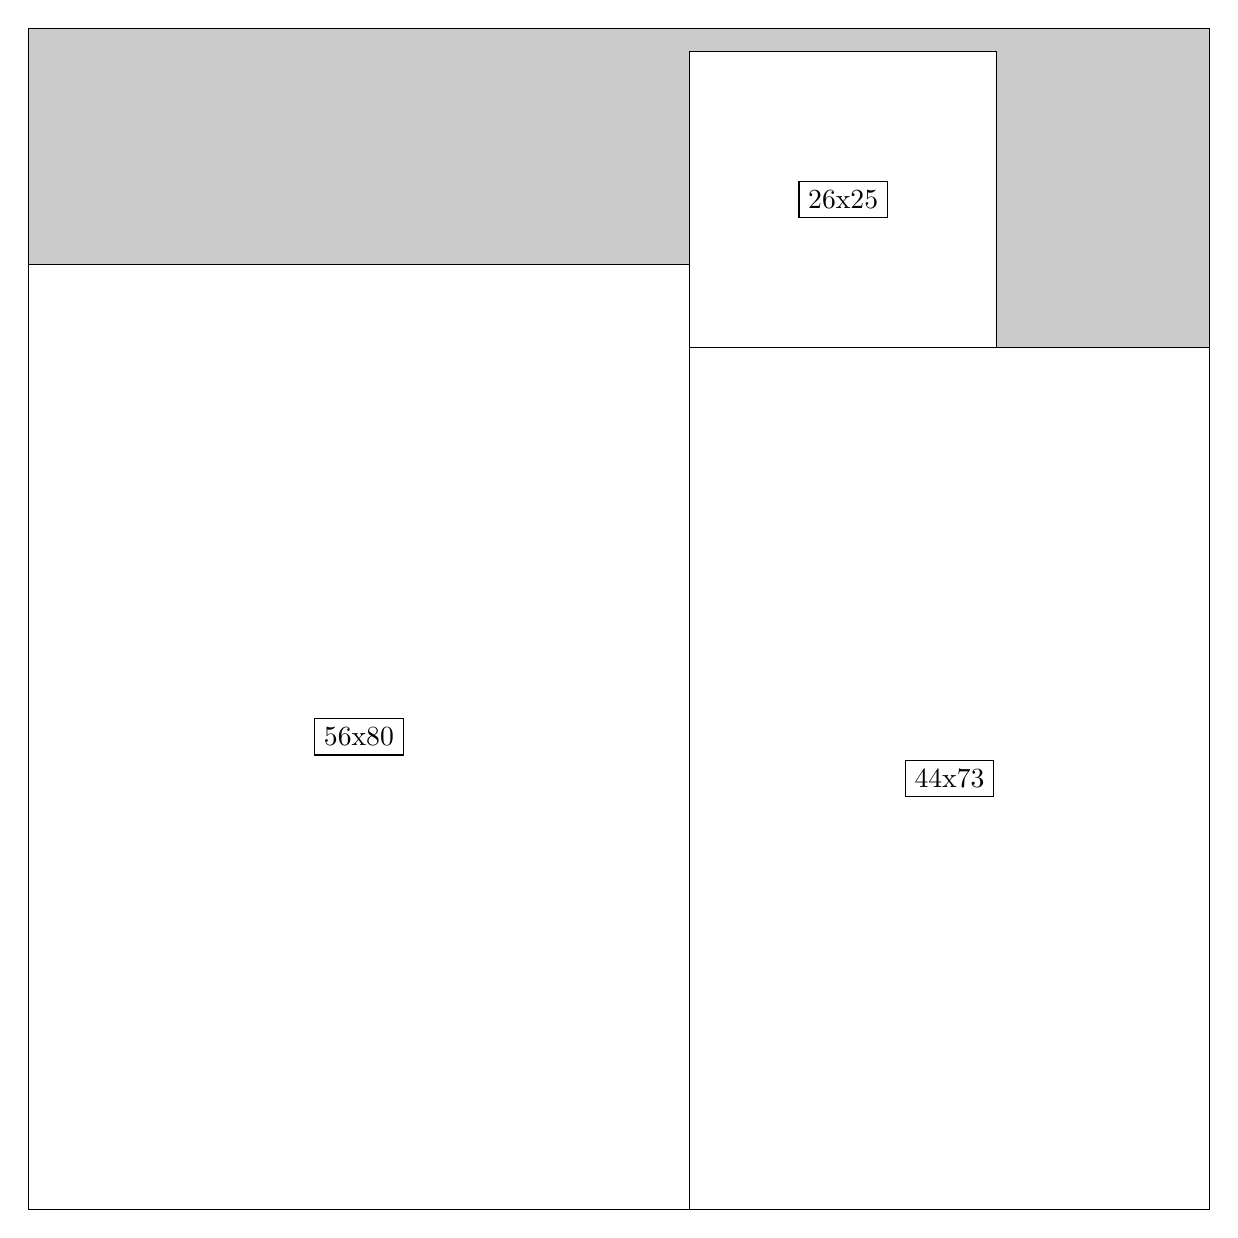
\begin{tikzpicture}[shorten >=1pt,scale=1.0,every node/.style={scale=1.0},->]
\tikzstyle{vertex}=[circle,fill=black!25,minimum size=14pt,inner sep=0pt]
\filldraw[fill=gray!40!white, draw=black] (0,0) rectangle (15.0,15.0);
\foreach \name/\x/\y/\w/\h in {56x80/0.0/0.0/8.4/12.0,44x73/8.4/0.0/6.6/10.95,26x25/8.4/10.95/3.9/3.75}
\filldraw[fill=white!40!white, draw=black] (\x,\y) rectangle node[draw] (\name) {\name} ++(\w,\h);
\end{tikzpicture}


w =56 , h =80 , x =0 , y =0 , v =4480
\par
w =44 , h =73 , x =56 , y =0 , v =3212
\par
w =26 , h =25 , x =56 , y =73 , v =650
\par
\newpage


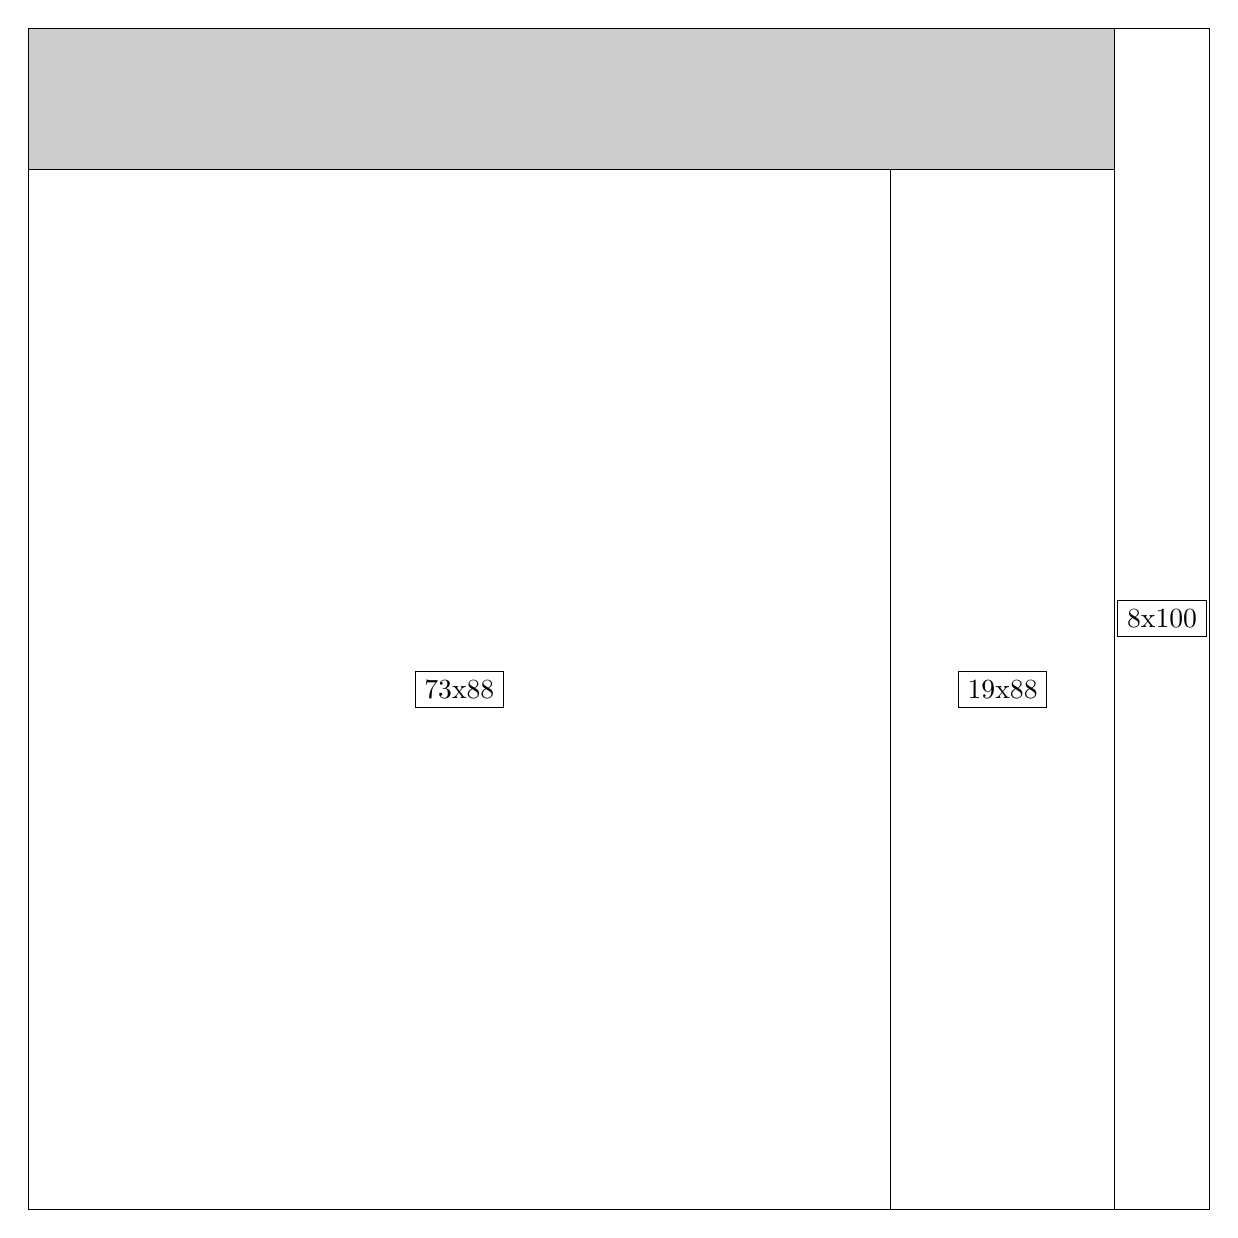
\begin{tikzpicture}[shorten >=1pt,scale=1.0,every node/.style={scale=1.0},->]
\tikzstyle{vertex}=[circle,fill=black!25,minimum size=14pt,inner sep=0pt]
\filldraw[fill=gray!40!white, draw=black] (0,0) rectangle (15.0,15.0);
\foreach \name/\x/\y/\w/\h in {19x88/10.95/0.0/2.85/13.2,73x88/0.0/0.0/10.95/13.2,8x100/13.799999999999999/0.0/1.2/15.0}
\filldraw[fill=white!40!white, draw=black] (\x,\y) rectangle node[draw] (\name) {\name} ++(\w,\h);
\end{tikzpicture}


w =19 , h =88 , x =73 , y =0 , v =1672
\par
w =73 , h =88 , x =0 , y =0 , v =6424
\par
w =8 , h =100 , x =92 , y =0 , v =800
\par
\newpage


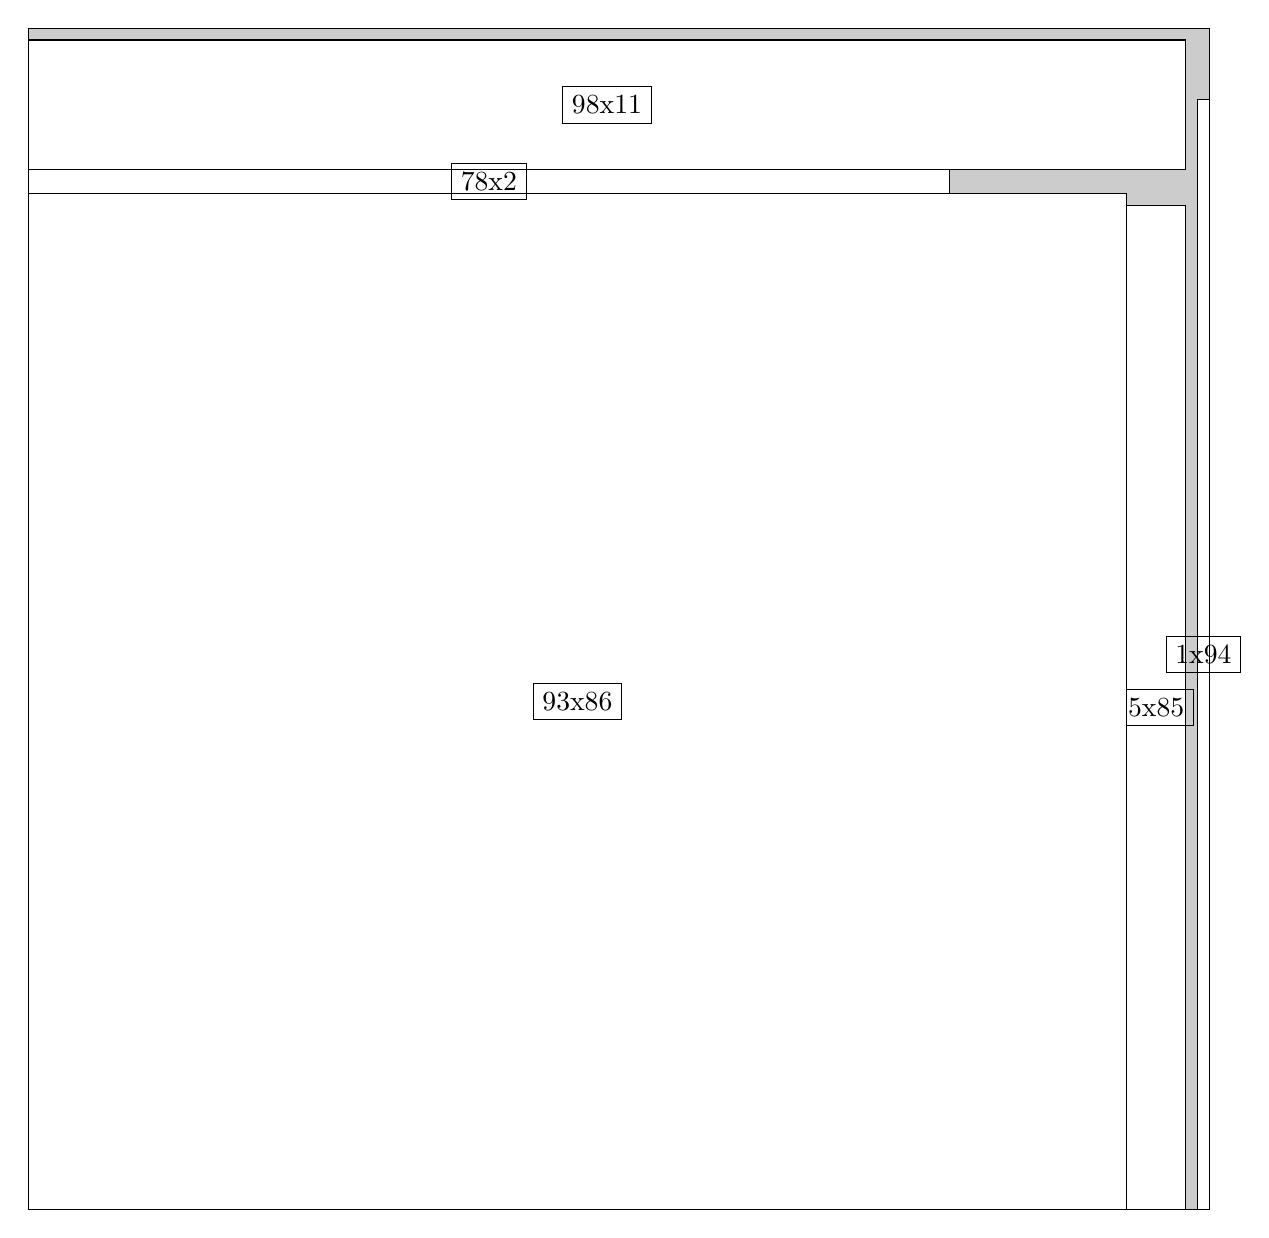
\begin{tikzpicture}[shorten >=1pt,scale=1.0,every node/.style={scale=1.0},->]
\tikzstyle{vertex}=[circle,fill=black!25,minimum size=14pt,inner sep=0pt]
\filldraw[fill=gray!40!white, draw=black] (0,0) rectangle (15.0,15.0);
\foreach \name/\x/\y/\w/\h in {5x85/13.95/0.0/0.75/12.75,93x86/0.0/0.0/13.95/12.9,98x11/0.0/13.2/14.7/1.65,78x2/0.0/12.9/11.7/0.3,1x94/14.85/0.0/0.15/14.1}
\filldraw[fill=white!40!white, draw=black] (\x,\y) rectangle node[draw] (\name) {\name} ++(\w,\h);
\end{tikzpicture}


w =5 , h =85 , x =93 , y =0 , v =425
\par
w =93 , h =86 , x =0 , y =0 , v =7998
\par
w =98 , h =11 , x =0 , y =88 , v =1078
\par
w =78 , h =2 , x =0 , y =86 , v =156
\par
w =1 , h =94 , x =99 , y =0 , v =94
\par
\newpage


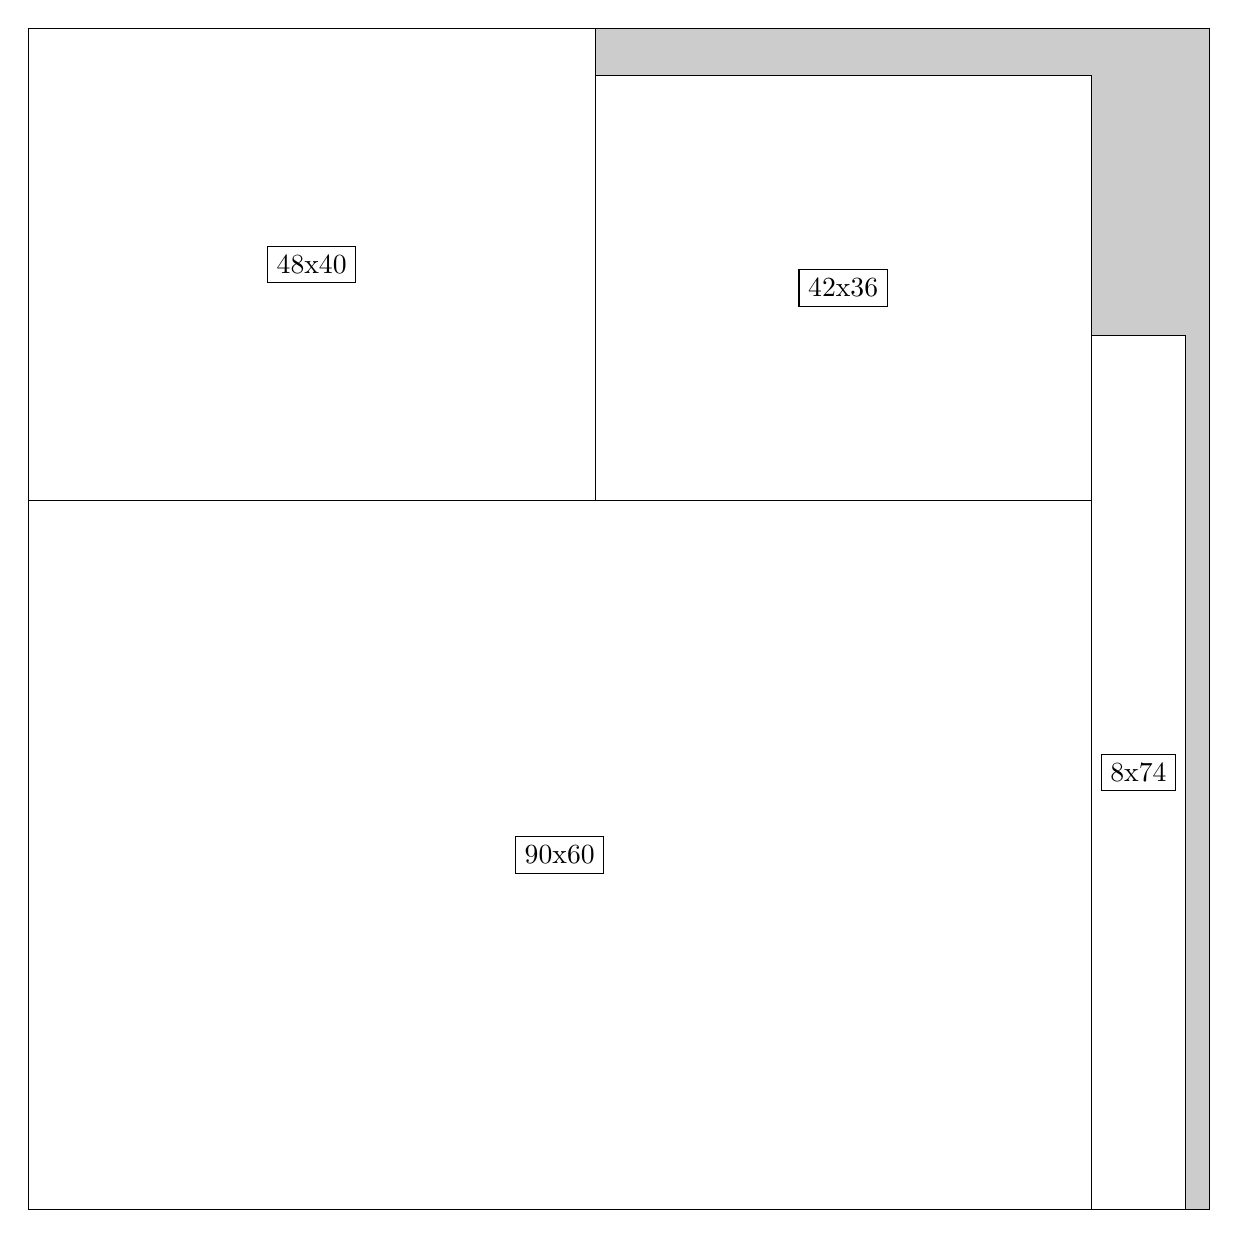
\begin{tikzpicture}[shorten >=1pt,scale=1.0,every node/.style={scale=1.0},->]
\tikzstyle{vertex}=[circle,fill=black!25,minimum size=14pt,inner sep=0pt]
\filldraw[fill=gray!40!white, draw=black] (0,0) rectangle (15.0,15.0);
\foreach \name/\x/\y/\w/\h in {48x40/0.0/9.0/7.199999999999999/6.0,90x60/0.0/0.0/13.5/9.0,8x74/13.5/0.0/1.2/11.1,42x36/7.199999999999999/9.0/6.3/5.3999999999999995}
\filldraw[fill=white!40!white, draw=black] (\x,\y) rectangle node[draw] (\name) {\name} ++(\w,\h);
\end{tikzpicture}


w =48 , h =40 , x =0 , y =60 , v =1920
\par
w =90 , h =60 , x =0 , y =0 , v =5400
\par
w =8 , h =74 , x =90 , y =0 , v =592
\par
w =42 , h =36 , x =48 , y =60 , v =1512
\par
\newpage


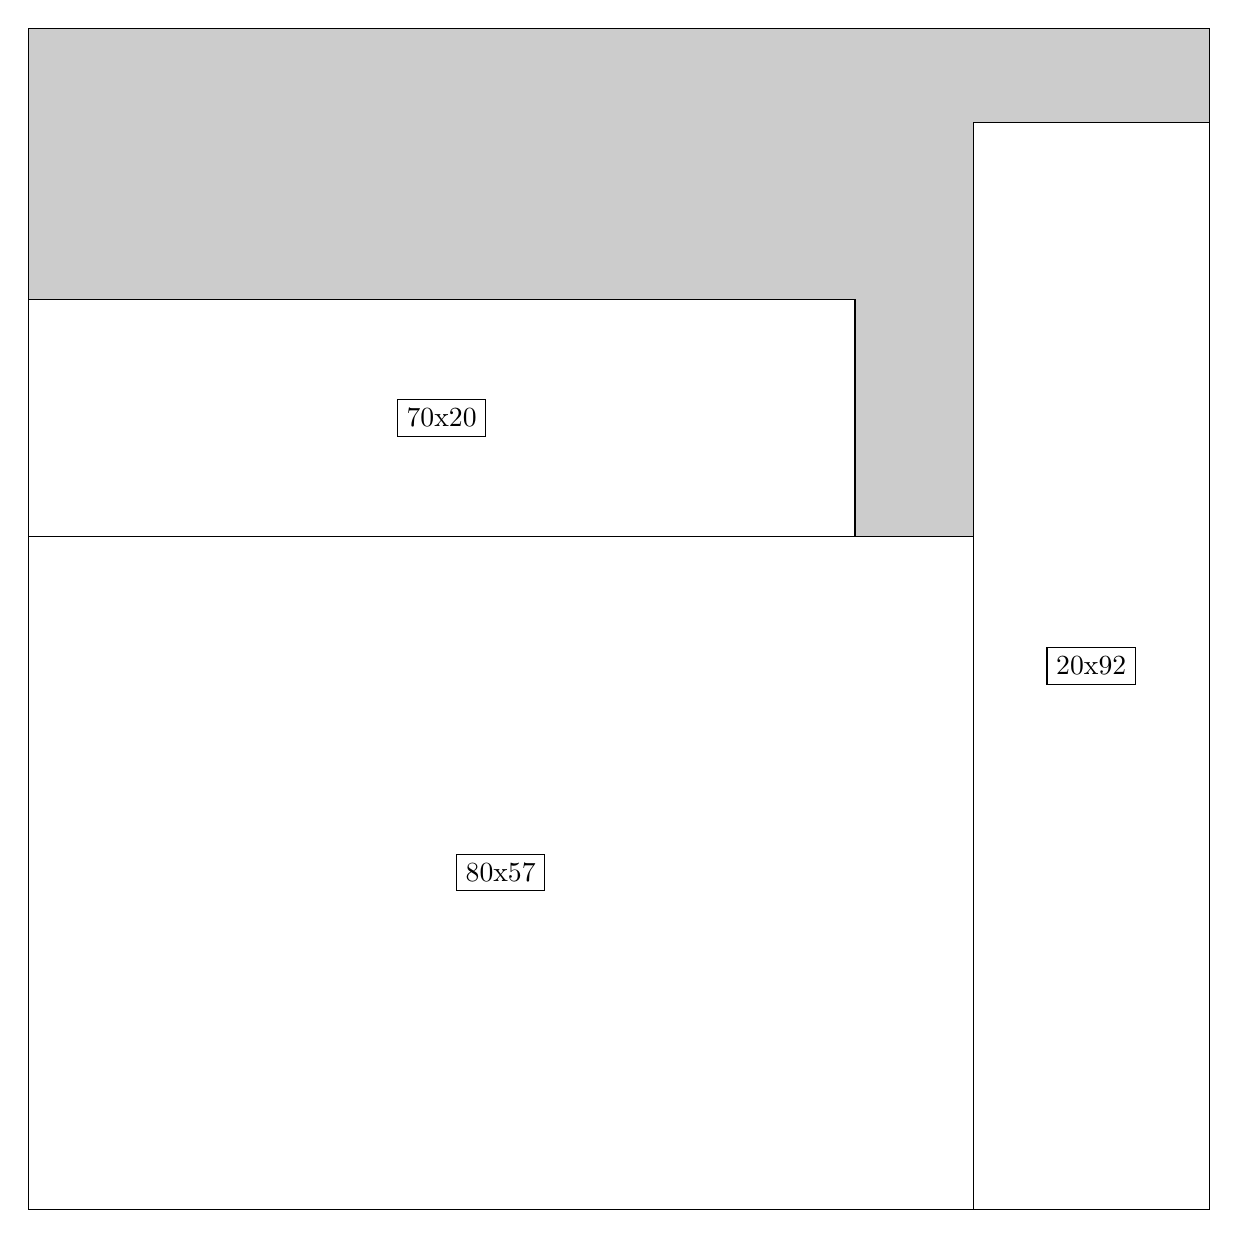
\begin{tikzpicture}[shorten >=1pt,scale=1.0,every node/.style={scale=1.0},->]
\tikzstyle{vertex}=[circle,fill=black!25,minimum size=14pt,inner sep=0pt]
\filldraw[fill=gray!40!white, draw=black] (0,0) rectangle (15.0,15.0);
\foreach \name/\x/\y/\w/\h in {20x92/12.0/0.0/3.0/13.799999999999999,80x57/0.0/0.0/12.0/8.549999999999999,70x20/0.0/8.549999999999999/10.5/3.0}
\filldraw[fill=white!40!white, draw=black] (\x,\y) rectangle node[draw] (\name) {\name} ++(\w,\h);
\end{tikzpicture}


w =20 , h =92 , x =80 , y =0 , v =1840
\par
w =80 , h =57 , x =0 , y =0 , v =4560
\par
w =70 , h =20 , x =0 , y =57 , v =1400
\par
\newpage


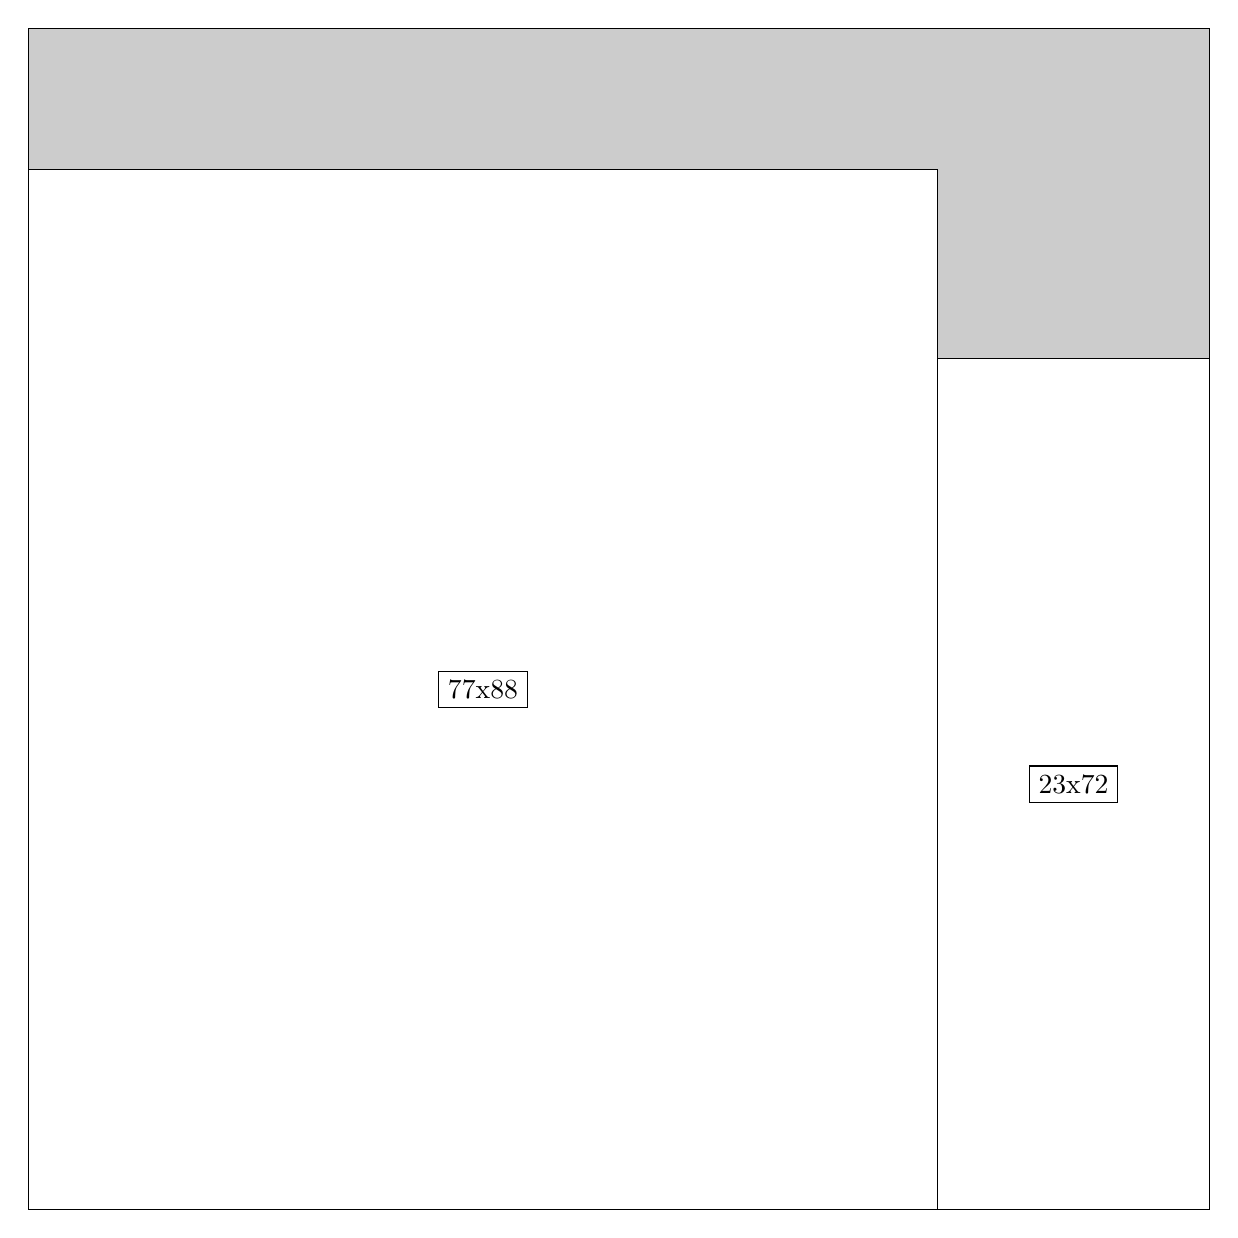
\begin{tikzpicture}[shorten >=1pt,scale=1.0,every node/.style={scale=1.0},->]
\tikzstyle{vertex}=[circle,fill=black!25,minimum size=14pt,inner sep=0pt]
\filldraw[fill=gray!40!white, draw=black] (0,0) rectangle (15.0,15.0);
\foreach \name/\x/\y/\w/\h in {23x72/11.549999999999999/0.0/3.4499999999999997/10.799999999999999,77x88/0.0/0.0/11.549999999999999/13.2}
\filldraw[fill=white!40!white, draw=black] (\x,\y) rectangle node[draw] (\name) {\name} ++(\w,\h);
\end{tikzpicture}


w =23 , h =72 , x =77 , y =0 , v =1656
\par
w =77 , h =88 , x =0 , y =0 , v =6776
\par
\newpage


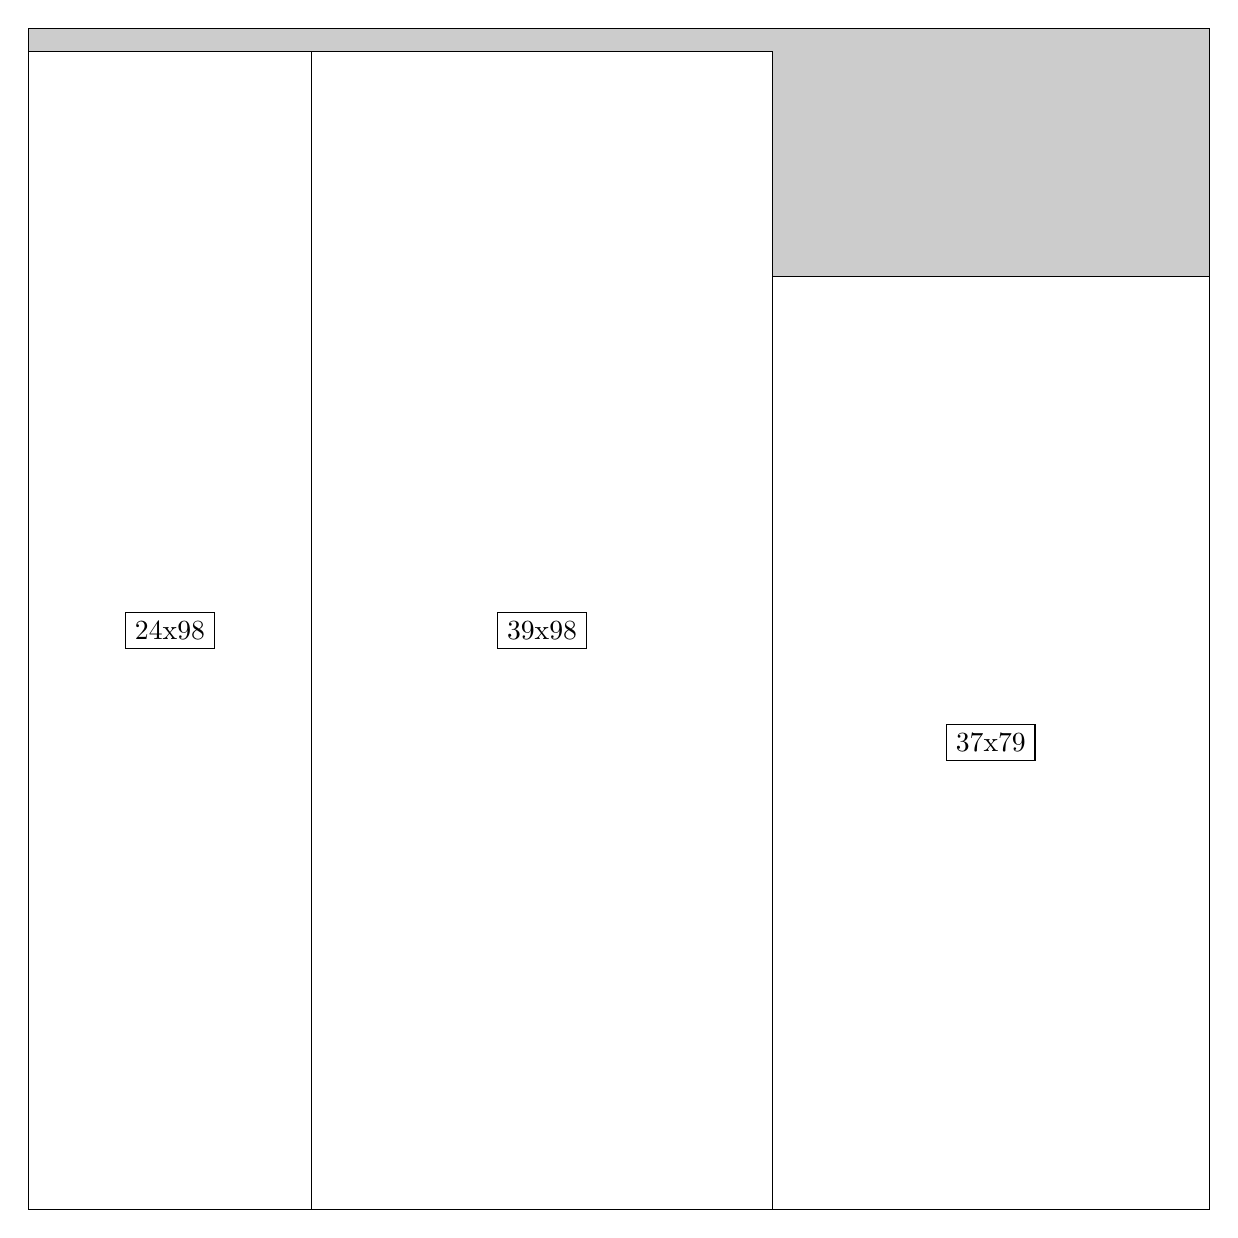
\begin{tikzpicture}[shorten >=1pt,scale=1.0,every node/.style={scale=1.0},->]
\tikzstyle{vertex}=[circle,fill=black!25,minimum size=14pt,inner sep=0pt]
\filldraw[fill=gray!40!white, draw=black] (0,0) rectangle (15.0,15.0);
\foreach \name/\x/\y/\w/\h in {24x98/0.0/0.0/3.5999999999999996/14.7,39x98/3.5999999999999996/0.0/5.85/14.7,37x79/9.45/0.0/5.55/11.85}
\filldraw[fill=white!40!white, draw=black] (\x,\y) rectangle node[draw] (\name) {\name} ++(\w,\h);
\end{tikzpicture}


w =24 , h =98 , x =0 , y =0 , v =2352
\par
w =39 , h =98 , x =24 , y =0 , v =3822
\par
w =37 , h =79 , x =63 , y =0 , v =2923
\par
\newpage


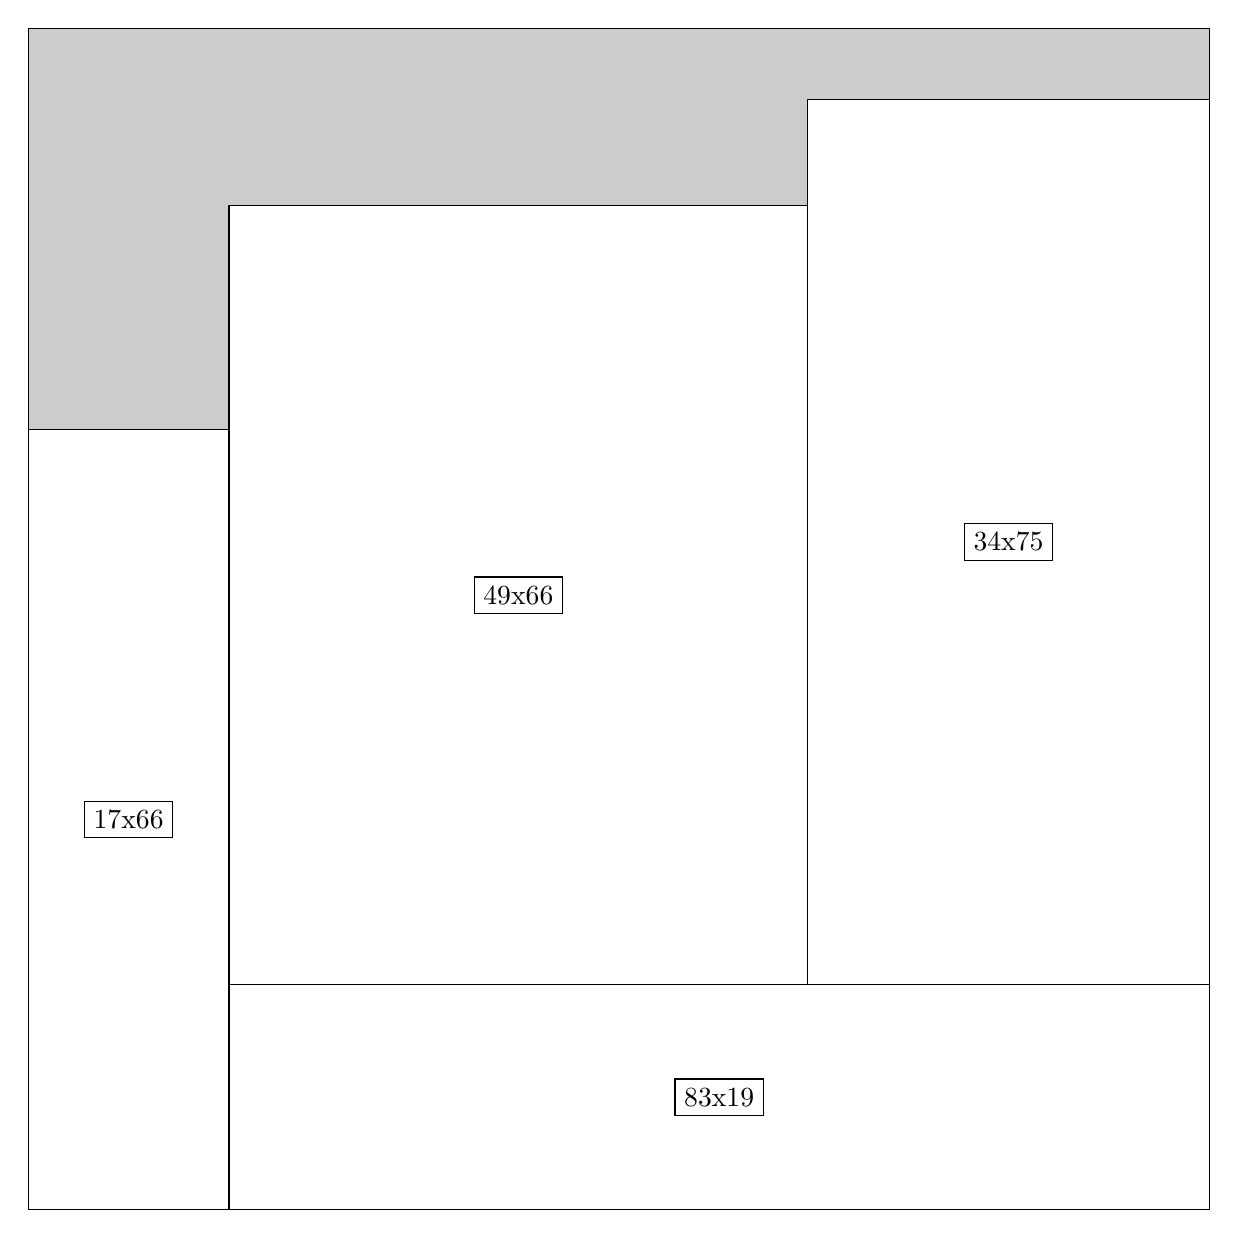
\begin{tikzpicture}[shorten >=1pt,scale=1.0,every node/.style={scale=1.0},->]
\tikzstyle{vertex}=[circle,fill=black!25,minimum size=14pt,inner sep=0pt]
\filldraw[fill=gray!40!white, draw=black] (0,0) rectangle (15.0,15.0);
\foreach \name/\x/\y/\w/\h in {17x66/0.0/0.0/2.55/9.9,49x66/2.55/2.85/7.35/9.9,83x19/2.55/0.0/12.45/2.85,34x75/9.9/2.85/5.1/11.25}
\filldraw[fill=white!40!white, draw=black] (\x,\y) rectangle node[draw] (\name) {\name} ++(\w,\h);
\end{tikzpicture}


w =17 , h =66 , x =0 , y =0 , v =1122
\par
w =49 , h =66 , x =17 , y =19 , v =3234
\par
w =83 , h =19 , x =17 , y =0 , v =1577
\par
w =34 , h =75 , x =66 , y =19 , v =2550
\par
\newpage


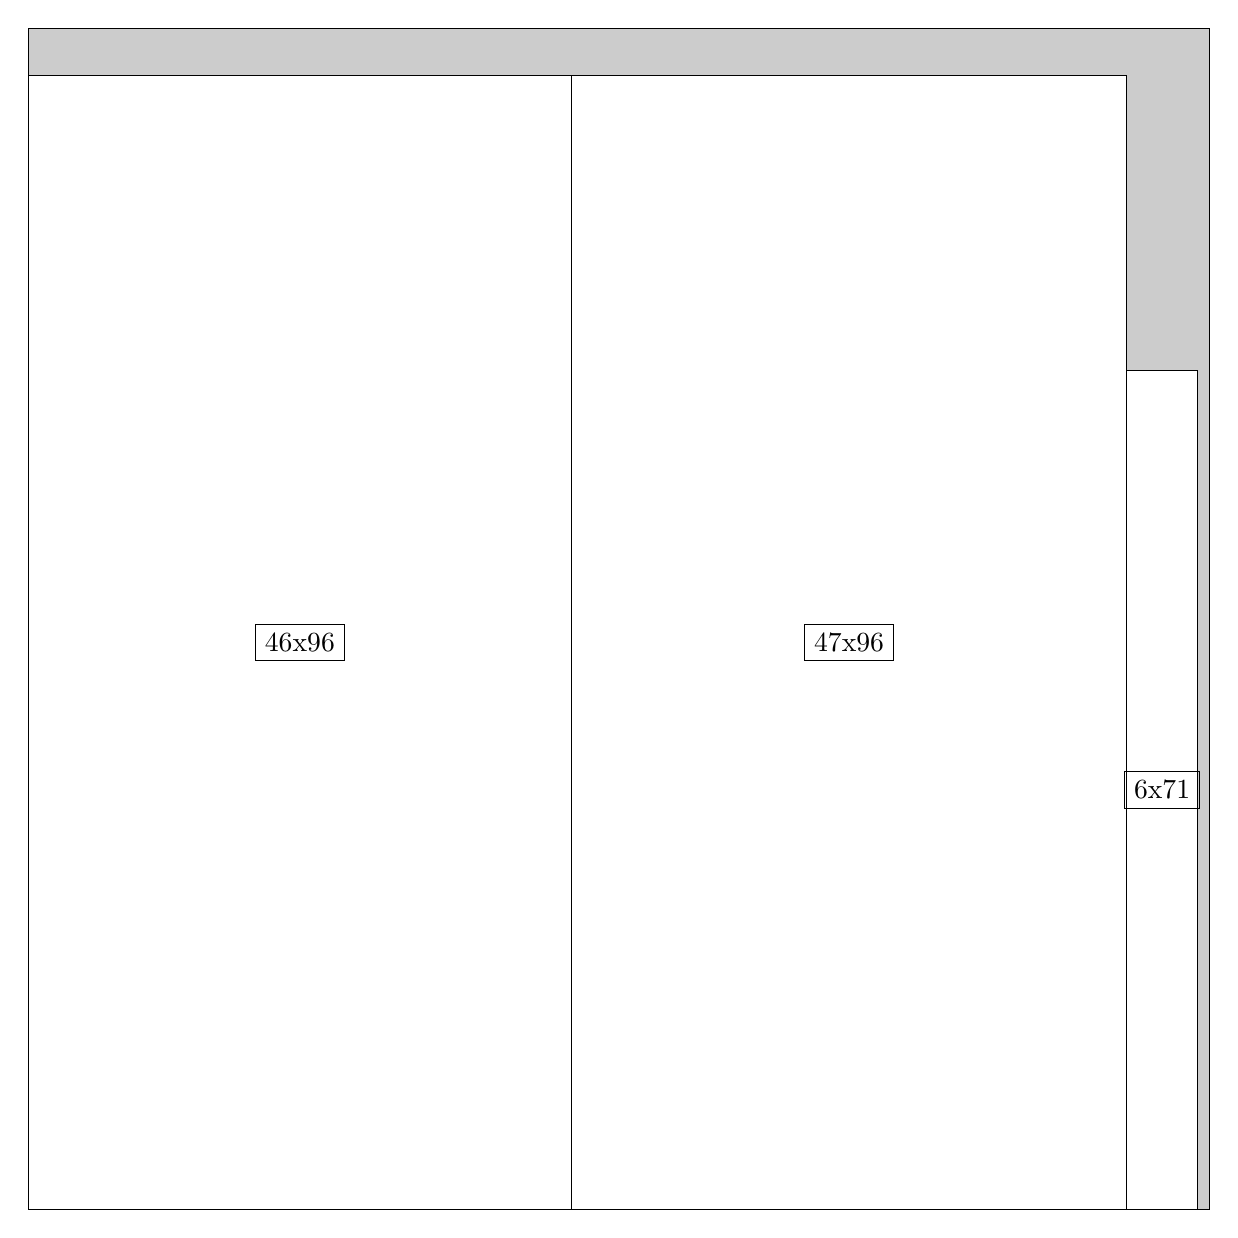
\begin{tikzpicture}[shorten >=1pt,scale=1.0,every node/.style={scale=1.0},->]
\tikzstyle{vertex}=[circle,fill=black!25,minimum size=14pt,inner sep=0pt]
\filldraw[fill=gray!40!white, draw=black] (0,0) rectangle (15.0,15.0);
\foreach \name/\x/\y/\w/\h in {46x96/0.0/0.0/6.8999999999999995/14.399999999999999,47x96/6.8999999999999995/0.0/7.05/14.399999999999999,6x71/13.95/0.0/0.8999999999999999/10.65}
\filldraw[fill=white!40!white, draw=black] (\x,\y) rectangle node[draw] (\name) {\name} ++(\w,\h);
\end{tikzpicture}


w =46 , h =96 , x =0 , y =0 , v =4416
\par
w =47 , h =96 , x =46 , y =0 , v =4512
\par
w =6 , h =71 , x =93 , y =0 , v =426
\par
\newpage


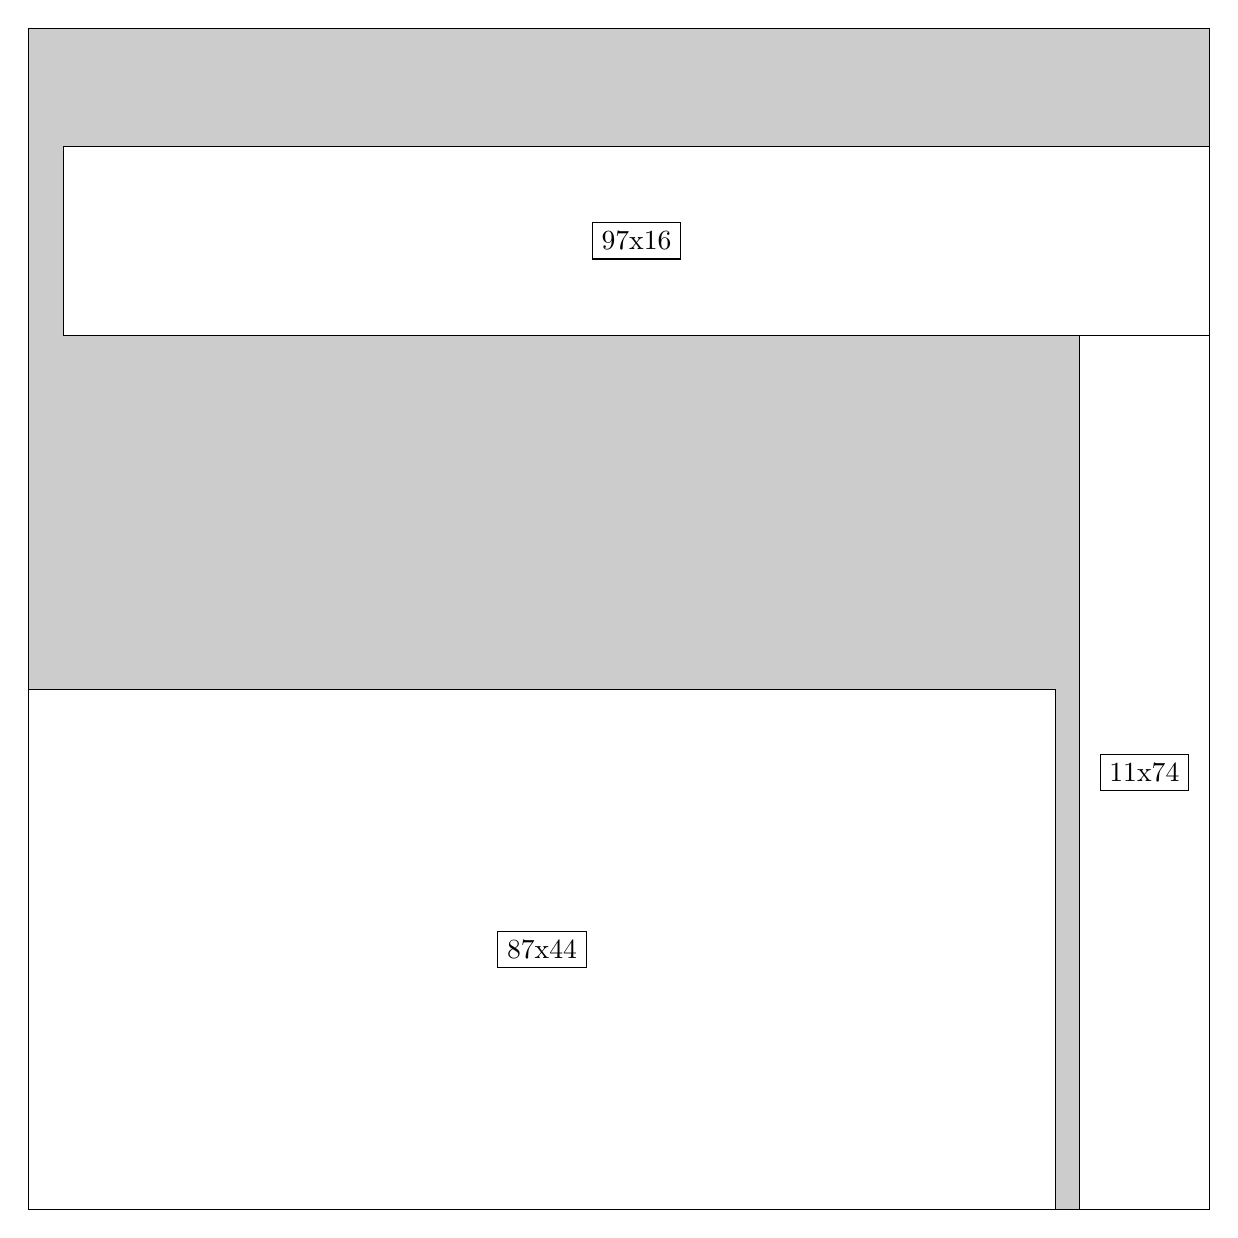
\begin{tikzpicture}[shorten >=1pt,scale=1.0,every node/.style={scale=1.0},->]
\tikzstyle{vertex}=[circle,fill=black!25,minimum size=14pt,inner sep=0pt]
\filldraw[fill=gray!40!white, draw=black] (0,0) rectangle (15.0,15.0);
\foreach \name/\x/\y/\w/\h in {87x44/0.0/0.0/13.049999999999999/6.6,97x16/0.44999999999999996/11.1/14.549999999999999/2.4,11x74/13.35/0.0/1.65/11.1}
\filldraw[fill=white!40!white, draw=black] (\x,\y) rectangle node[draw] (\name) {\name} ++(\w,\h);
\end{tikzpicture}


w =87 , h =44 , x =0 , y =0 , v =3828
\par
w =97 , h =16 , x =3 , y =74 , v =1552
\par
w =11 , h =74 , x =89 , y =0 , v =814
\par
\newpage


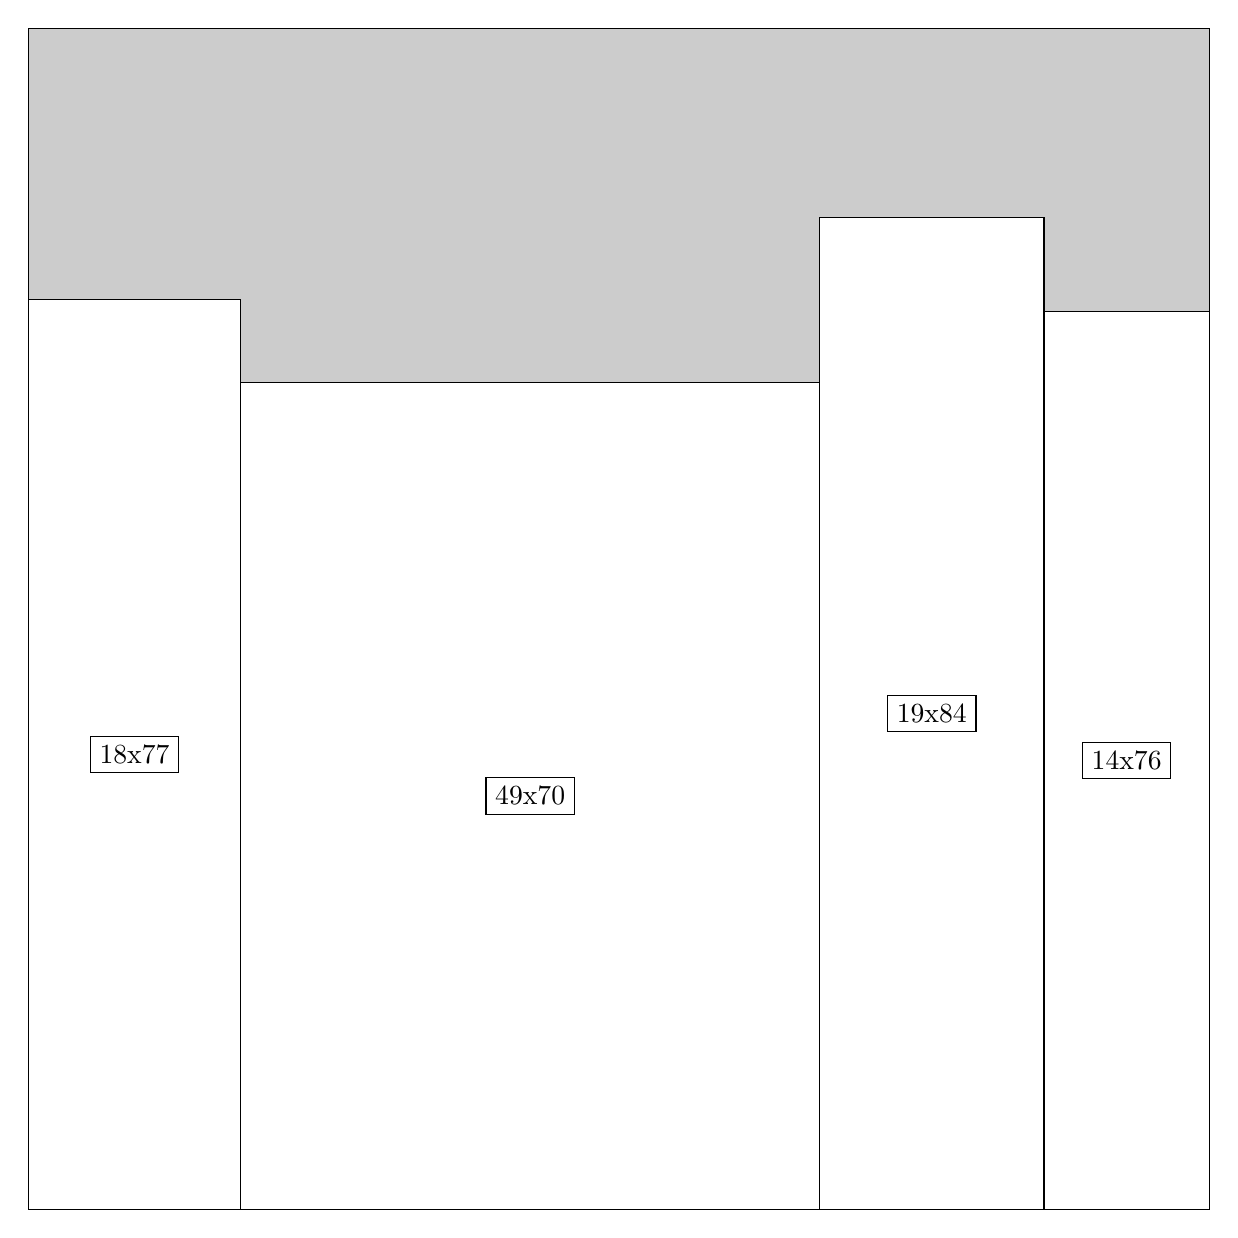
\begin{tikzpicture}[shorten >=1pt,scale=1.0,every node/.style={scale=1.0},->]
\tikzstyle{vertex}=[circle,fill=black!25,minimum size=14pt,inner sep=0pt]
\filldraw[fill=gray!40!white, draw=black] (0,0) rectangle (15.0,15.0);
\foreach \name/\x/\y/\w/\h in {18x77/0.0/0.0/2.6999999999999997/11.549999999999999,49x70/2.6999999999999997/0.0/7.35/10.5,19x84/10.049999999999999/0.0/2.85/12.6,14x76/12.9/0.0/2.1/11.4}
\filldraw[fill=white!40!white, draw=black] (\x,\y) rectangle node[draw] (\name) {\name} ++(\w,\h);
\end{tikzpicture}


w =18 , h =77 , x =0 , y =0 , v =1386
\par
w =49 , h =70 , x =18 , y =0 , v =3430
\par
w =19 , h =84 , x =67 , y =0 , v =1596
\par
w =14 , h =76 , x =86 , y =0 , v =1064
\par
\newpage


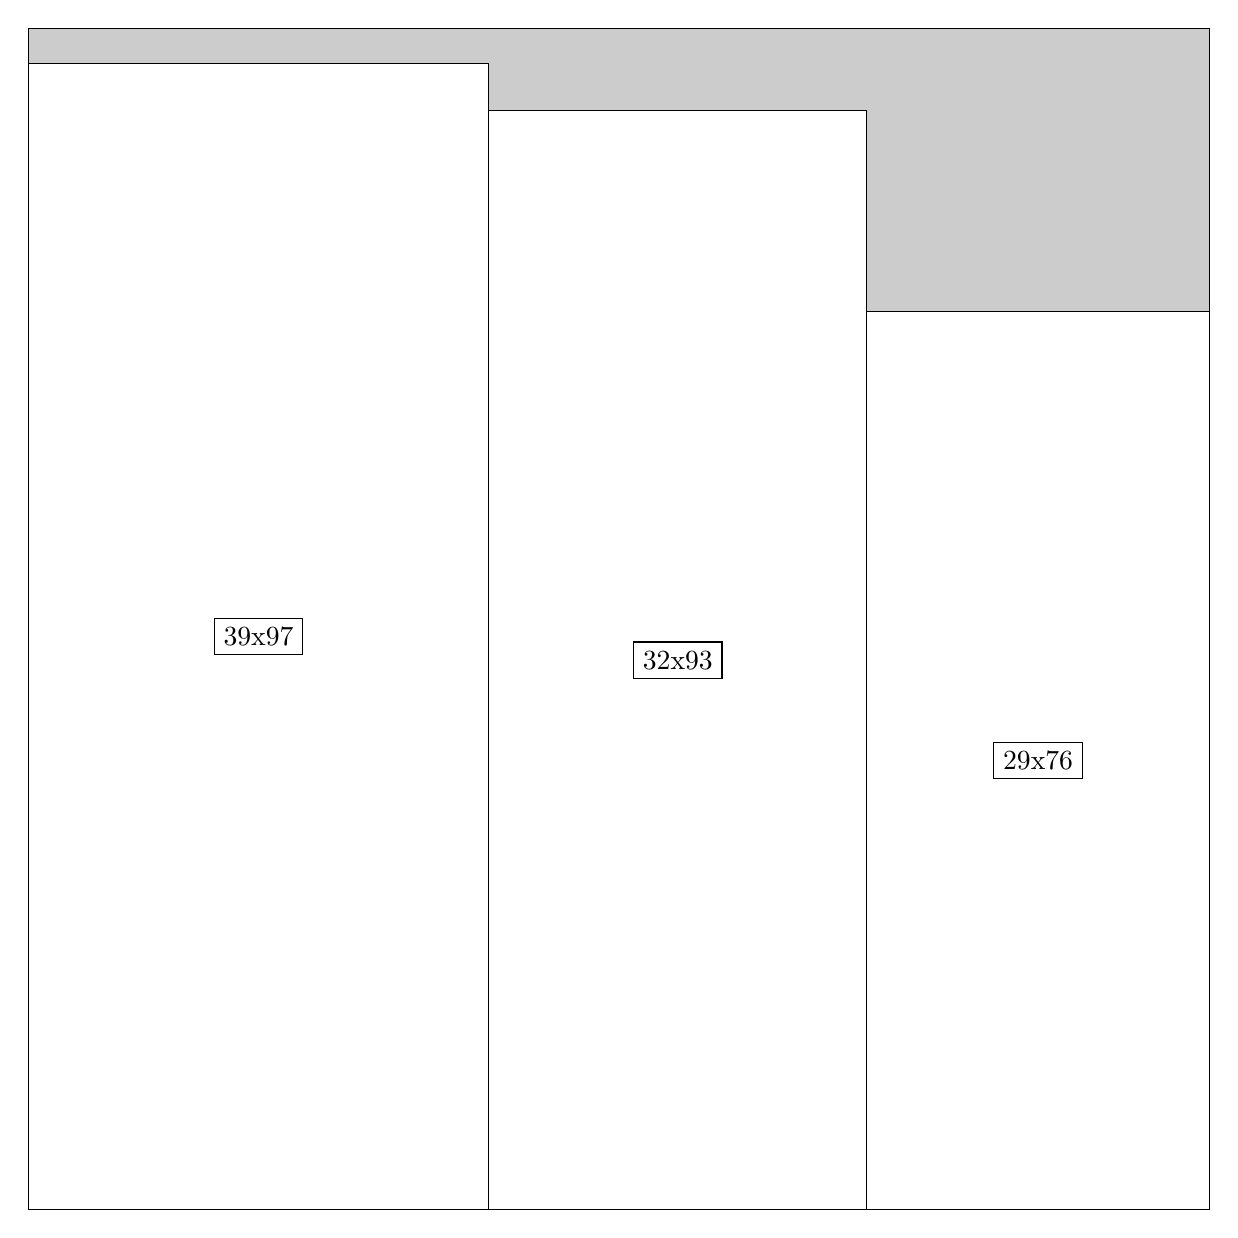
\begin{tikzpicture}[shorten >=1pt,scale=1.0,every node/.style={scale=1.0},->]
\tikzstyle{vertex}=[circle,fill=black!25,minimum size=14pt,inner sep=0pt]
\filldraw[fill=gray!40!white, draw=black] (0,0) rectangle (15.0,15.0);
\foreach \name/\x/\y/\w/\h in {39x97/0.0/0.0/5.85/14.549999999999999,32x93/5.85/0.0/4.8/13.95,29x76/10.65/0.0/4.35/11.4}
\filldraw[fill=white!40!white, draw=black] (\x,\y) rectangle node[draw] (\name) {\name} ++(\w,\h);
\end{tikzpicture}


w =39 , h =97 , x =0 , y =0 , v =3783
\par
w =32 , h =93 , x =39 , y =0 , v =2976
\par
w =29 , h =76 , x =71 , y =0 , v =2204
\par
\newpage


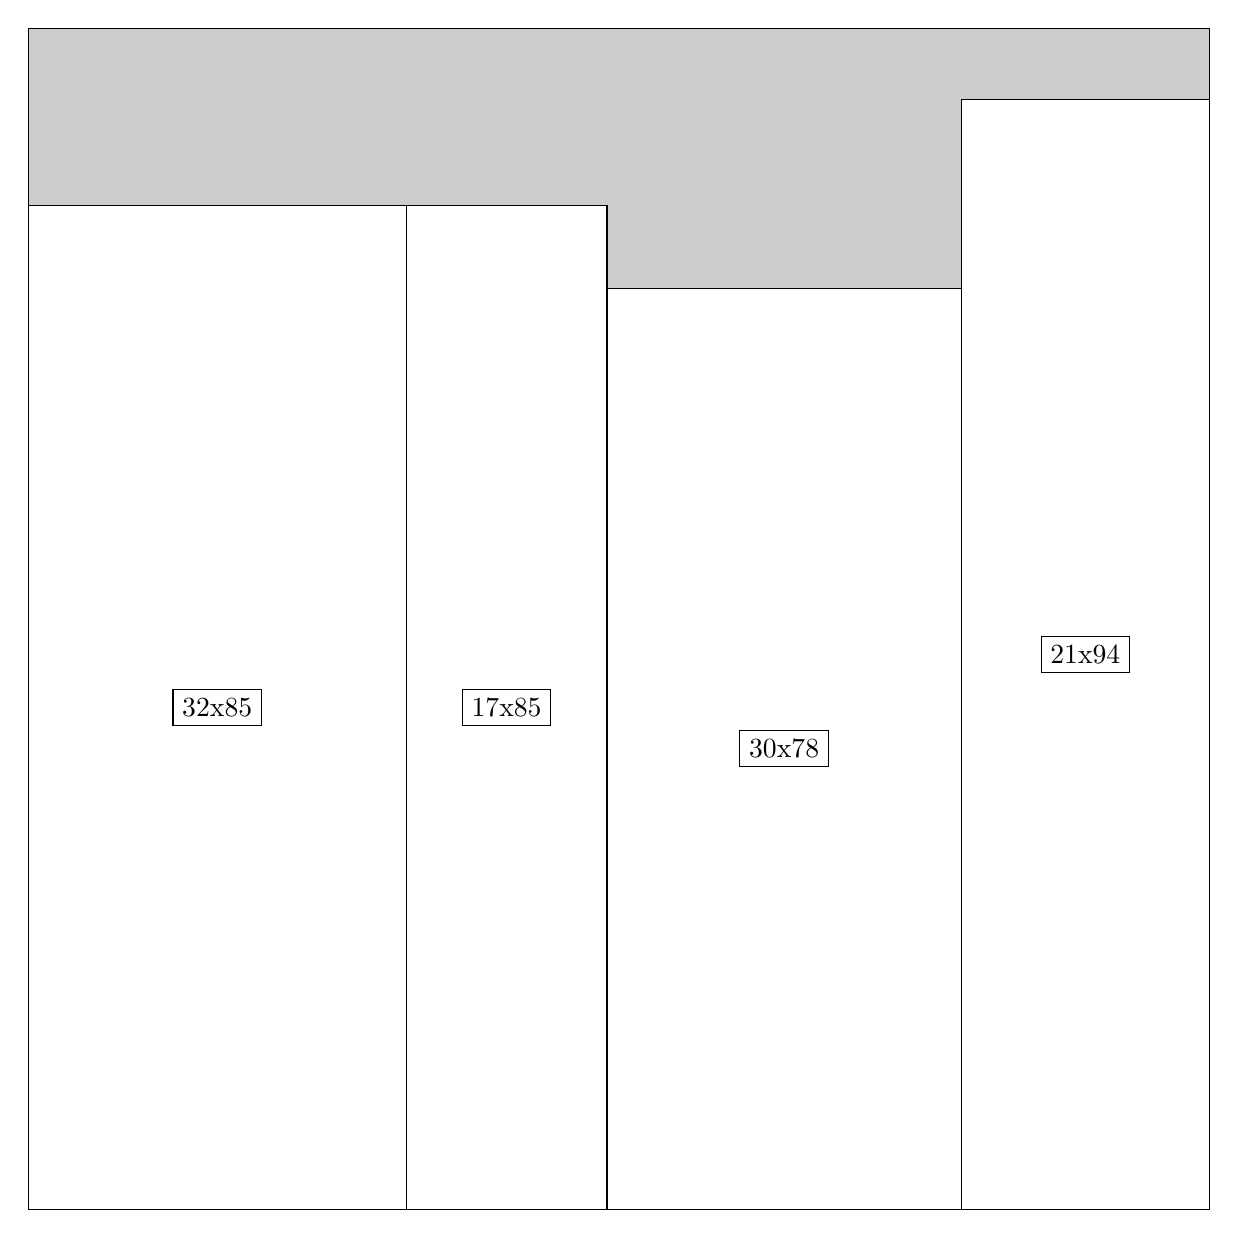
\begin{tikzpicture}[shorten >=1pt,scale=1.0,every node/.style={scale=1.0},->]
\tikzstyle{vertex}=[circle,fill=black!25,minimum size=14pt,inner sep=0pt]
\filldraw[fill=gray!40!white, draw=black] (0,0) rectangle (15.0,15.0);
\foreach \name/\x/\y/\w/\h in {32x85/0.0/0.0/4.8/12.75,30x78/7.35/0.0/4.5/11.7,21x94/11.85/0.0/3.15/14.1,17x85/4.8/0.0/2.55/12.75}
\filldraw[fill=white!40!white, draw=black] (\x,\y) rectangle node[draw] (\name) {\name} ++(\w,\h);
\end{tikzpicture}


w =32 , h =85 , x =0 , y =0 , v =2720
\par
w =30 , h =78 , x =49 , y =0 , v =2340
\par
w =21 , h =94 , x =79 , y =0 , v =1974
\par
w =17 , h =85 , x =32 , y =0 , v =1445
\par
\newpage


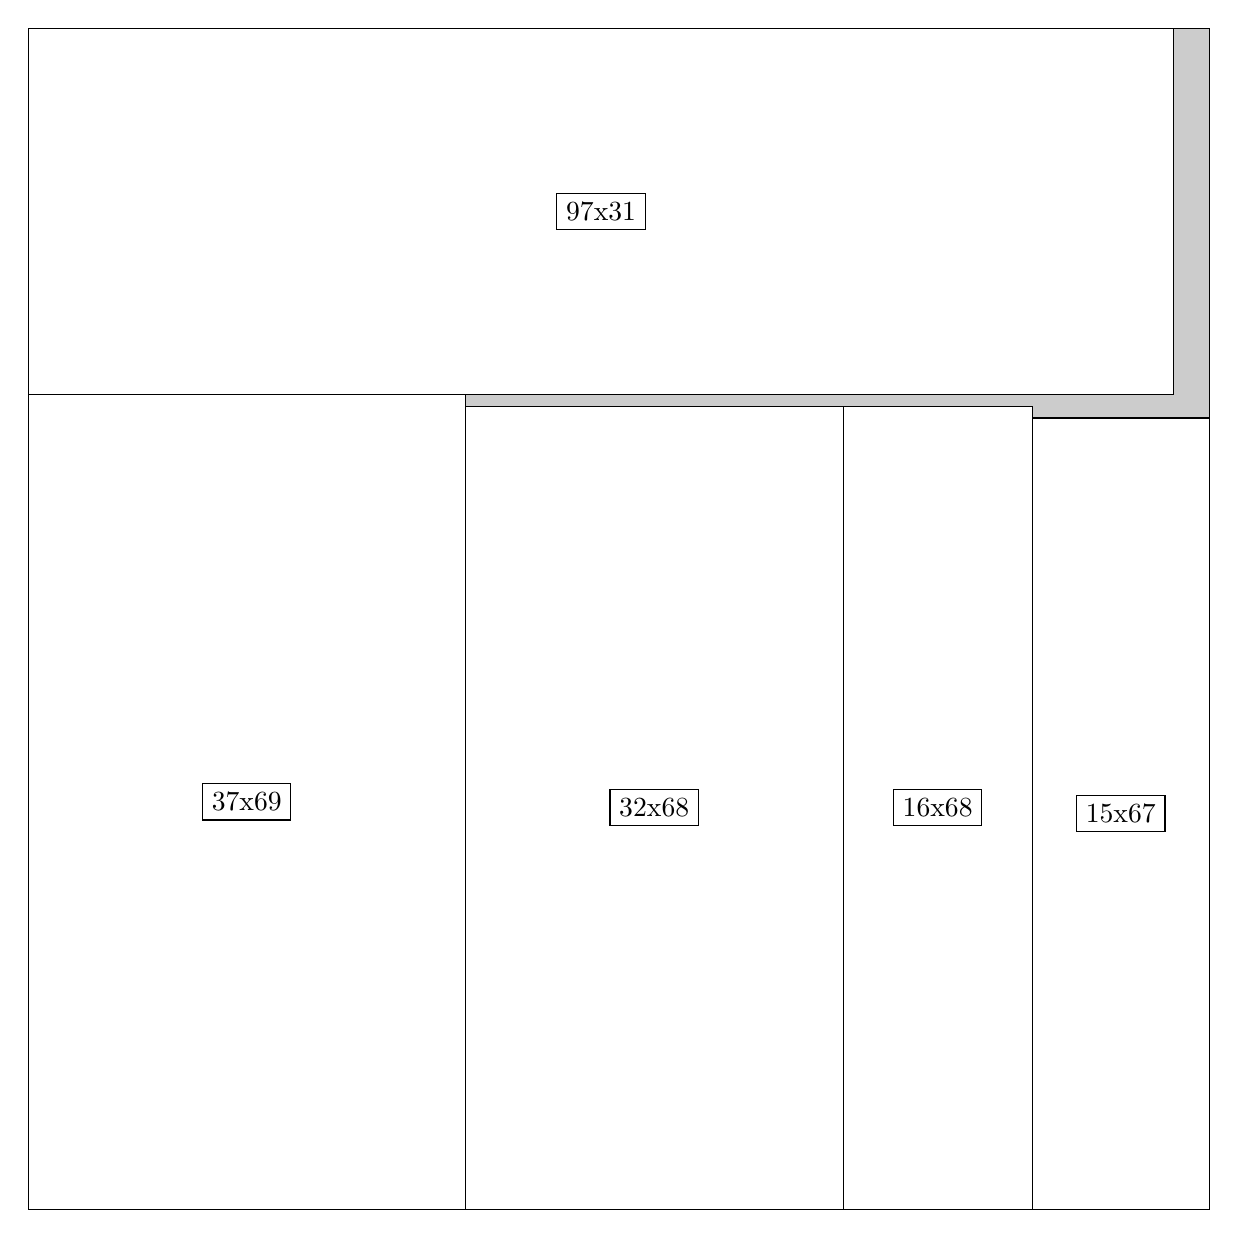
\begin{tikzpicture}[shorten >=1pt,scale=1.0,every node/.style={scale=1.0},->]
\tikzstyle{vertex}=[circle,fill=black!25,minimum size=14pt,inner sep=0pt]
\filldraw[fill=gray!40!white, draw=black] (0,0) rectangle (15.0,15.0);
\foreach \name/\x/\y/\w/\h in {37x69/0.0/0.0/5.55/10.35,32x68/5.55/0.0/4.8/10.2,97x31/0.0/10.35/14.549999999999999/4.6499999999999995,15x67/12.75/0.0/2.25/10.049999999999999,16x68/10.35/0.0/2.4/10.2}
\filldraw[fill=white!40!white, draw=black] (\x,\y) rectangle node[draw] (\name) {\name} ++(\w,\h);
\end{tikzpicture}


w =37 , h =69 , x =0 , y =0 , v =2553
\par
w =32 , h =68 , x =37 , y =0 , v =2176
\par
w =97 , h =31 , x =0 , y =69 , v =3007
\par
w =15 , h =67 , x =85 , y =0 , v =1005
\par
w =16 , h =68 , x =69 , y =0 , v =1088
\par
\newpage


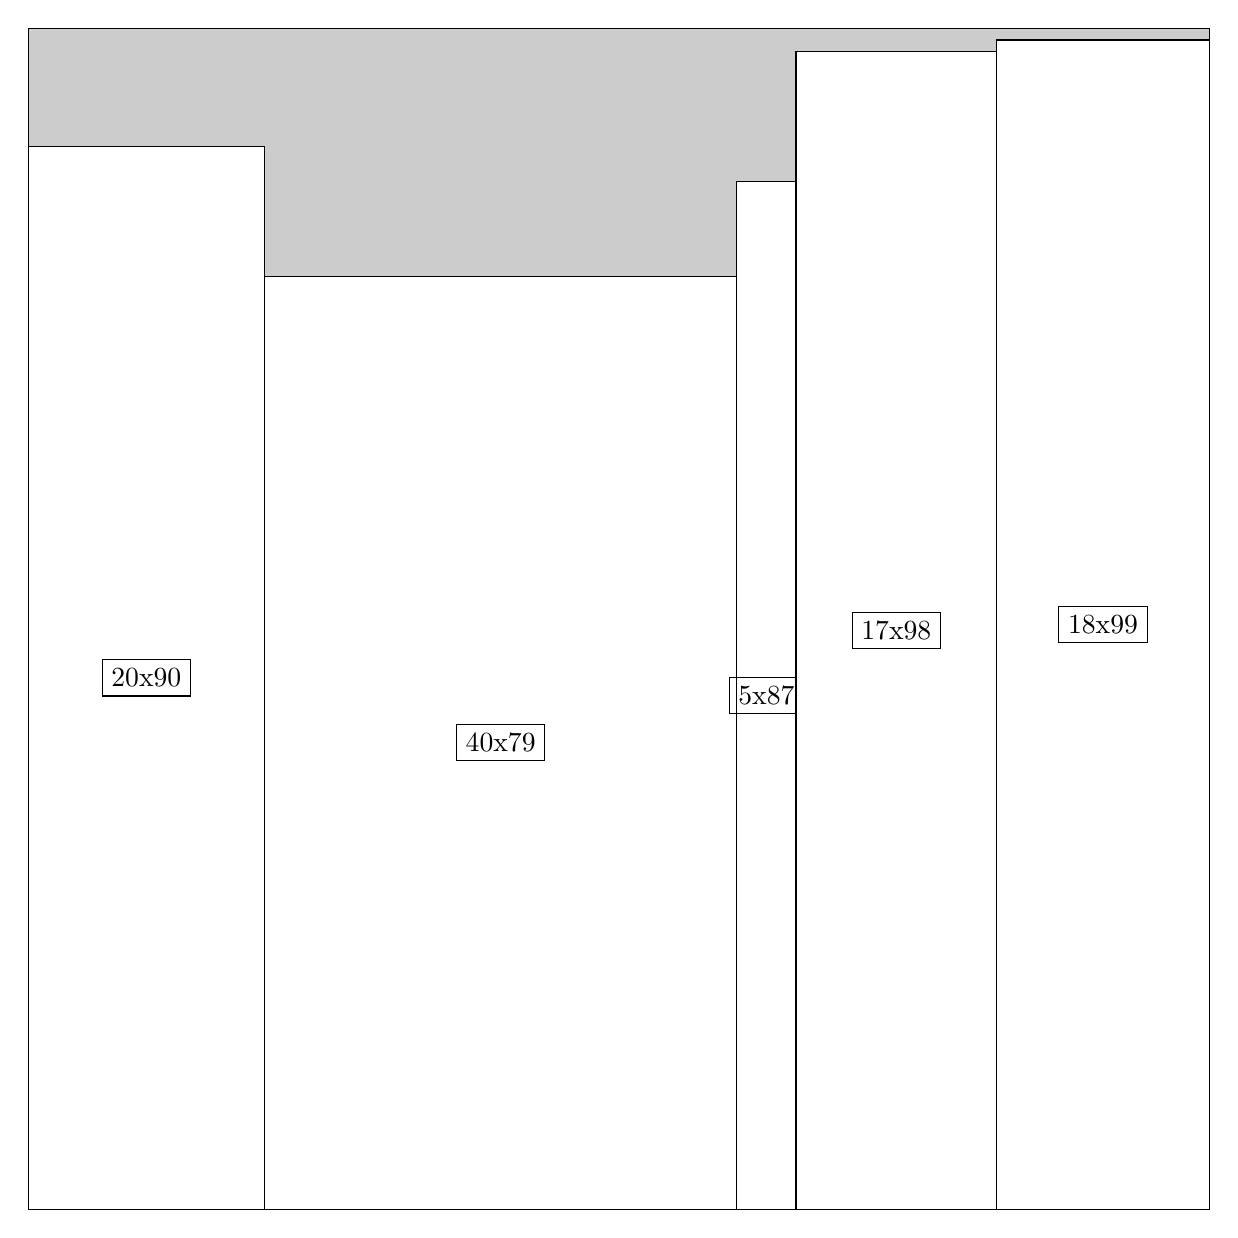
\begin{tikzpicture}[shorten >=1pt,scale=1.0,every node/.style={scale=1.0},->]
\tikzstyle{vertex}=[circle,fill=black!25,minimum size=14pt,inner sep=0pt]
\filldraw[fill=gray!40!white, draw=black] (0,0) rectangle (15.0,15.0);
\foreach \name/\x/\y/\w/\h in {18x99/12.299999999999999/0.0/2.6999999999999997/14.85,20x90/0.0/0.0/3.0/13.5,40x79/3.0/0.0/6.0/11.85,5x87/9.0/0.0/0.75/13.049999999999999,17x98/9.75/0.0/2.55/14.7}
\filldraw[fill=white!40!white, draw=black] (\x,\y) rectangle node[draw] (\name) {\name} ++(\w,\h);
\end{tikzpicture}


w =18 , h =99 , x =82 , y =0 , v =1782
\par
w =20 , h =90 , x =0 , y =0 , v =1800
\par
w =40 , h =79 , x =20 , y =0 , v =3160
\par
w =5 , h =87 , x =60 , y =0 , v =435
\par
w =17 , h =98 , x =65 , y =0 , v =1666
\par
\newpage


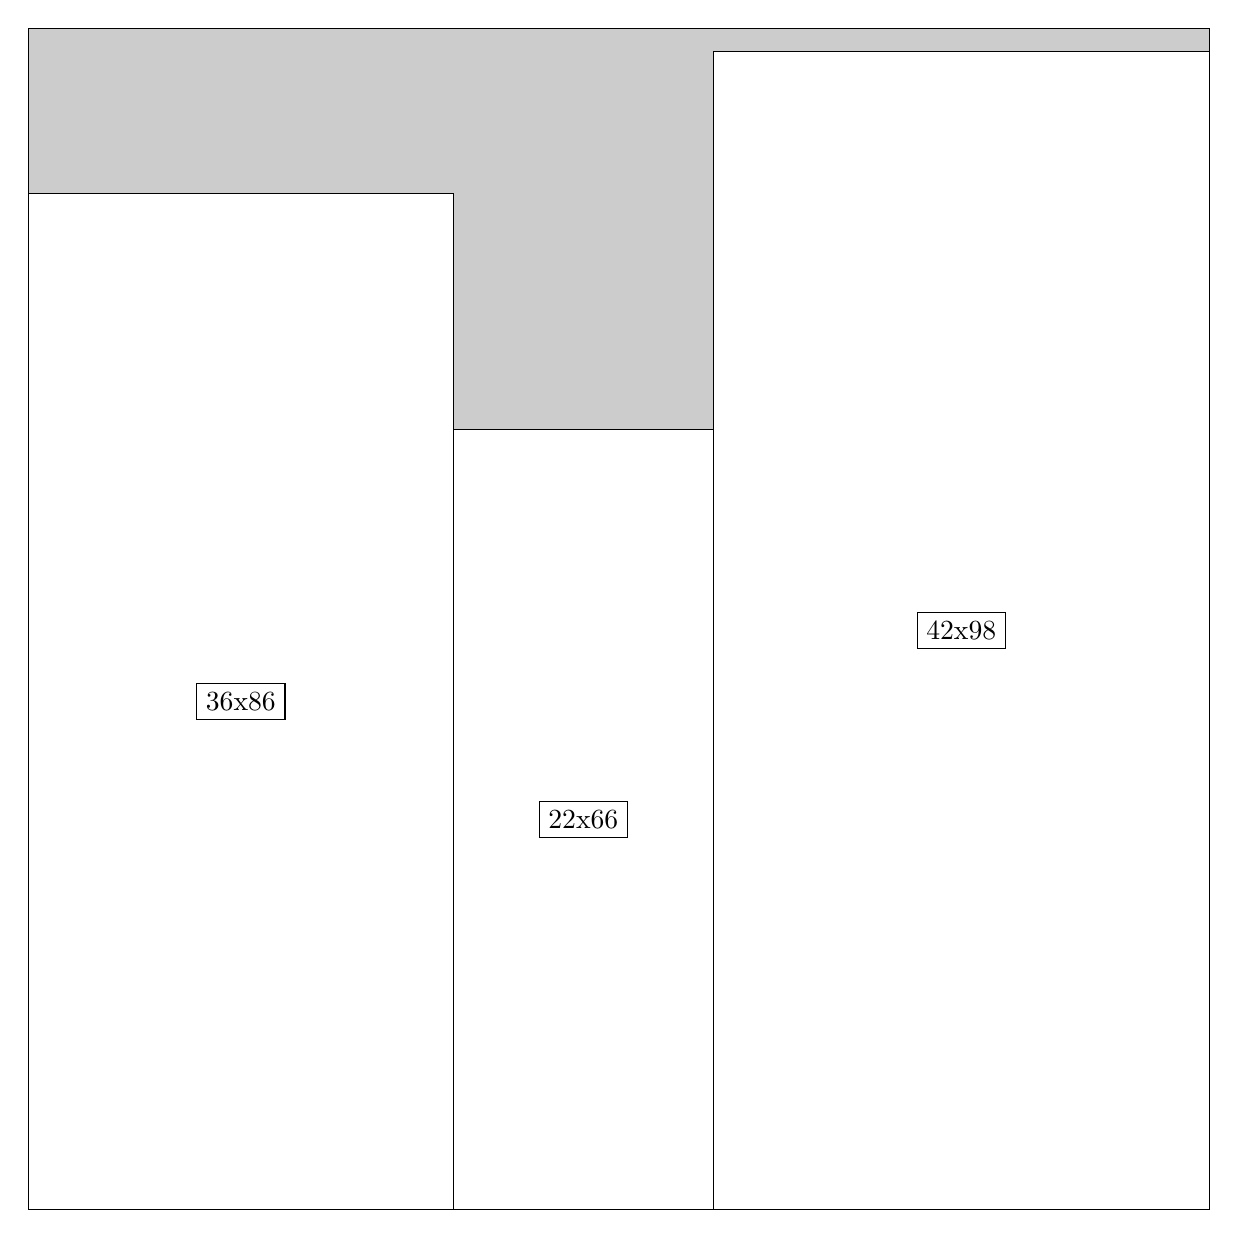
\begin{tikzpicture}[shorten >=1pt,scale=1.0,every node/.style={scale=1.0},->]
\tikzstyle{vertex}=[circle,fill=black!25,minimum size=14pt,inner sep=0pt]
\filldraw[fill=gray!40!white, draw=black] (0,0) rectangle (15.0,15.0);
\foreach \name/\x/\y/\w/\h in {36x86/0.0/0.0/5.3999999999999995/12.9,22x66/5.3999999999999995/0.0/3.3/9.9,42x98/8.7/0.0/6.3/14.7}
\filldraw[fill=white!40!white, draw=black] (\x,\y) rectangle node[draw] (\name) {\name} ++(\w,\h);
\end{tikzpicture}


w =36 , h =86 , x =0 , y =0 , v =3096
\par
w =22 , h =66 , x =36 , y =0 , v =1452
\par
w =42 , h =98 , x =58 , y =0 , v =4116
\par
\newpage


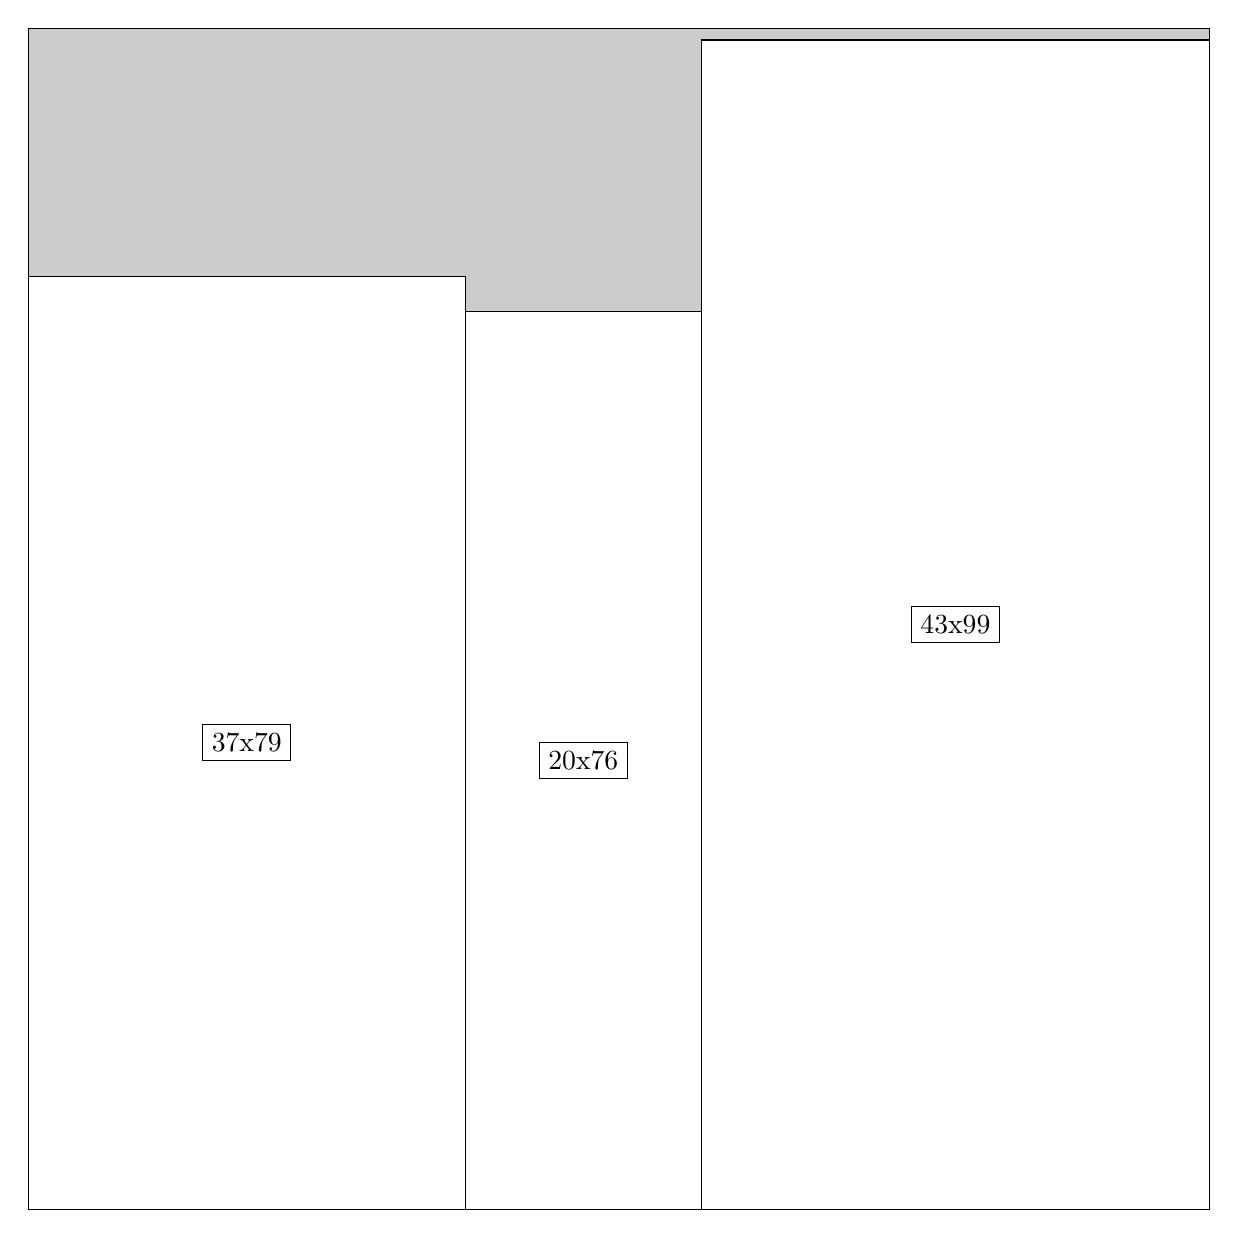
\begin{tikzpicture}[shorten >=1pt,scale=1.0,every node/.style={scale=1.0},->]
\tikzstyle{vertex}=[circle,fill=black!25,minimum size=14pt,inner sep=0pt]
\filldraw[fill=gray!40!white, draw=black] (0,0) rectangle (15.0,15.0);
\foreach \name/\x/\y/\w/\h in {37x79/0.0/0.0/5.55/11.85,43x99/8.549999999999999/0.0/6.45/14.85,20x76/5.55/0.0/3.0/11.4}
\filldraw[fill=white!40!white, draw=black] (\x,\y) rectangle node[draw] (\name) {\name} ++(\w,\h);
\end{tikzpicture}


w =37 , h =79 , x =0 , y =0 , v =2923
\par
w =43 , h =99 , x =57 , y =0 , v =4257
\par
w =20 , h =76 , x =37 , y =0 , v =1520
\par
\newpage


\end{document}